 
 \begin{figure}
        \centerline{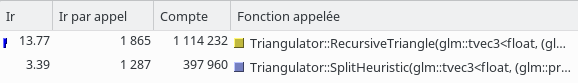
\includegraphics[width=8cm]{img/noCullingVal.png}}
        \caption{Le cout du frustum Culling}
        \label{fig:perfNoCulling}
 \end{figure}
 
 \begin{figure}
        \centerline{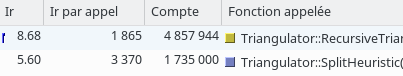
\includegraphics[width=8cm]{img/cullingAfterFixValgrind.png}}
        \caption{Division}
        \label{fig:perfCulling}
 \end{figure}
 Les 2 captures d'écrans \ref{fig:perfNoCulling} et \ref{fig:perfCulling} montrent à quel point le mode SplitCull est plus consommateur que le mode normal.  Les sorties ont été réalisées en s'assurant que tous les triangles de la récursion soient au niveau de détails 2, la caméra centrée sur la planète. Le frustum culling ne sert donc à rien dans ces conditions.
 
 
 Pour la sortie 1, sans culling, la branche de récursion est donc :
 \newline
 Split->Leaf.

Pour l'autre, avec culling:
 \newline
 SplitCull->Leaf.
 
 On se rend compte que le mode culling a demander 3 fois plus d'instructions.
 